%See notion notes for very rough outline of possible research approach
%----------| section  outline |----------%
 The goal of this proposed thesis is to develop a three-dimensional, model-based, closed-loop dynamic controller for continuous soft robots. This proposal would now like to put forward a breakdown of how research in pursuit of the goal will be approached. The work shall be conducted in three phases: the Model Selection phase, Model Calibration phase, and finally the Controller Implementation phase, these phases are described below.   
%----------| 1. Formulation, augmentation, or selection of a dynamics model
\subsection{Model Selection}
%<-- WHY! Need to outline and highlight benefits of contemporary models
This proposal has discussed the importance and impacts of the constitutive dynamical model used when designing model-based controllers, and consequently how limitations born out of the model's assumptions can translate to implementation challenges in the controller. The Model Selection phase has been included in the research approach in light of this, specifically in the interest of making the development of the controller as practical as possible.

The majority of this phase has been and will continue to be dedicated to reviewing the body of literature available. We are particularly interested in identifying models that can be applied to rod-like continuous soft robots, but also models that possess at least one of the two following characteristics: 1) a model with some precedent of implementing a controller for it, or 2) a model whose underlying dynamic assumptions, kinematics, and/or parametrization has been shown to be robust. The models from \cite{della_santina_model-based_2020} and \cite{della_santina_improved_2020} previously discussed in this proposal belong to each category, respectively. We preliminarily present a tabulated summary of our current findings in \autoref{modelsum} below.

\begin{table}[!h]
    \begin{tabularx}{\textwidth}{|*{4}{>{\centering\arraybackslash}X|}}
        \hline
        Model & \# of States & ODE? & Controller?\\ \hline
        Augmented Rigid Body \cite{della_santina_model-based_2020} & $3$ & Yes, but only within certain boundaries & Yes \\ \hline
        Arc-Length Parametrization \cite{della_santina_improved_2020} & 3 (5*) \par *(parametric states) & Yes & Yes \\ \hline
        Discrete Cosserat Approach \cite{renda_discrete_2018} & 6 & No* \par *(solved via recursive algorithms) & No \\ \hline
    \end{tabularx}
    \caption{Characteristics and features of the dynamic models reviewed so far}
    \label{modelsum}
\end{table}

Through this literature review, the author hopes to gain a better view of what the prevailing dynamic models being used in the field are. The main goal of this phase is to identify \textit{a} model whose feasibility regarding the design of a controller for it falls within the time scope of the proposed thesis. This proposal would like to stress that the main focus of the proposed thesis is \textit{not} dynamical modelling of soft robots, but rather \textit{controller design} for them. As such, we are more interested in designing around a "workable" model than identifying \textit{the} perfect model.    
%----------| 2. Model validation
\subsection{Model Calibration}
Since one of the goals of this proposed thesis is to validate the controller designed via hardware implementation, the chosen dynamic model will need to be tuned to the test bench platform we have at hand (see \autoref{soroimg}). Practically speaking, this means evaluating what the various dynamical terms and matrices are for our soft robot.

\begin{figure}[!ht]
    \centering
    \includegraphics[width=0.6\textwidth]{graphics/limb.jpg}
    \caption{The 3-D pneumatically-actuated "limb" serving as our test bench platform}
    \label{soroimg}
\end{figure}

From the construction and physical characteristics of the robot alone, some semblance of what the dynamical terms and matrices of the robot are can be extracted. This initial application of the model to our system can be considered the "un-tuned" model. It can then be tuned by motor-babbling (passing in a series of randomized inputs--"babbles") our soft robot, simulate motor-babbling the soft robot \textit{using} the model, and then comparing the outputs between the two. Generally speaking, a "perfect" model would simulate an exact replica of the output that the robot itself physically produced. While the tuned model cannot do the same, it should simulate sufficiently accurate outputs when operating in configurations found within the boundaries established by the model's assumptions.

\begin{comment}
    \begin{figure}[!ht]
        \begin{subfigure}{0.3\textwidth}
            \subcaption{}
        \end{subfigure}
        \begin{subfigure}{0.3\textwidth}
            \subcaption{}
        \end{subfigure}
        \begin{subfigure}{0.3\textwidth}
            \subcaption{}
        \end{subfigure}
        \caption{An illustration comparing how the motor-babbling outputs would be simulated by a) the un-tuned model, b) a "perfect" model, and c) the tuned model}
        \label{varoutputs}
    \end{figure}
\end{comment}

The main goal of this phase is to calibrate the dynamic model to such an extent that it can sufficiently represent how the system \textit{responds} to an input signal. Since our soft robot is \textit{pneumatically}-actuated, that means the input signal will be in terms of pressure change. Roughly speaking, we want to ensure that for a given pressure change, the model simulates a change in configuration reflective of the change in configuration physically exhibited by the robot.   
%----------| 3. Control development, implementation, and validation
\subsection{Controller Implementation}
The goal of this phase is to arrive at a formulation for the controller, physically implement it on our test bench platform, and finally assess the controller's performance. The type of model determines how the controller ends up being formulated but assuming we end up moving forward with a PCC-based model, then the system can be considered as a Langragian system whose dynamics can be expressed in the standard form (see \autoref{eq:dynamics}).

\begin{equation}
    \mathbf{B}(\underline{q})\underline{\ddot{q}} + \mathbf{C}(\underline{q},\underline{\dot{q}})\underline{\dot{q}} + \mathbf{K}\underline{q} + \mathbf{D}\underline{\dot{q}} = \mathbf{A}(\underline{q})\underline{u}
    \label{eq:dynamics}
\end{equation}
Here, $\underline{q}$ is the configuration vector, $\mathbf{B}$ is the inertia matrix, $\mathbf{C}$ is the matrix collecting Coriolis and centrifugal forces, $\mathbf{K}$ is the elasticity matrix, $\mathbf{D}$ is the damping matrix, and $\mathbf{A}$ maps the input $\underline{u}$ into wrenches.
\begin{comment}
    The phase will be initiated by first formulating the controller using known theories and current literature. This will consume the majority of the phase, as some amount of research into the body of literature available regarding controller design for the chosen model specifically will need to be done. Any reviews of theories or concepts deemed necessary at this point will also need to be conducted. 
\end{comment}
In both \cite{della_santina_model-based_2020} and \cite{della_santina_improved_2020} where this formulation was used, similar methodologies were used to subsequently arrive at the controller:
\begin{equation}
    \label{eq:controller}
    \begin{split}
        \underline{u} &= \mathbf{A}^{-1}(-\mathbf{B}\underline{\ddot{q}}_{ref} - \mathbf{C}\underline{\dot{q}}_{ref} - \mathbf{K}\underline{q}_{ref}\\
        &- \mathbf{D}\underline{\dot{q}}_{ref} + \mathbf{K}_p(\underline{q}_{ref}-\underline{q}) - \mathbf{K}_D(\underline{\dot{q}}_{ref}-\underline{\dot{q}}))
    \end{split}
\end{equation}

Our controller will be designed following the framework outlined in the works mentioned above, with the main functionality to be pursued being task-space regulation and then trajectory tracking. Then preliminary validation of the controller will be conducted via simulation before a more thorough experimentation is conducted on hardware.   

\begin{figure}[!ht]
    \centering
    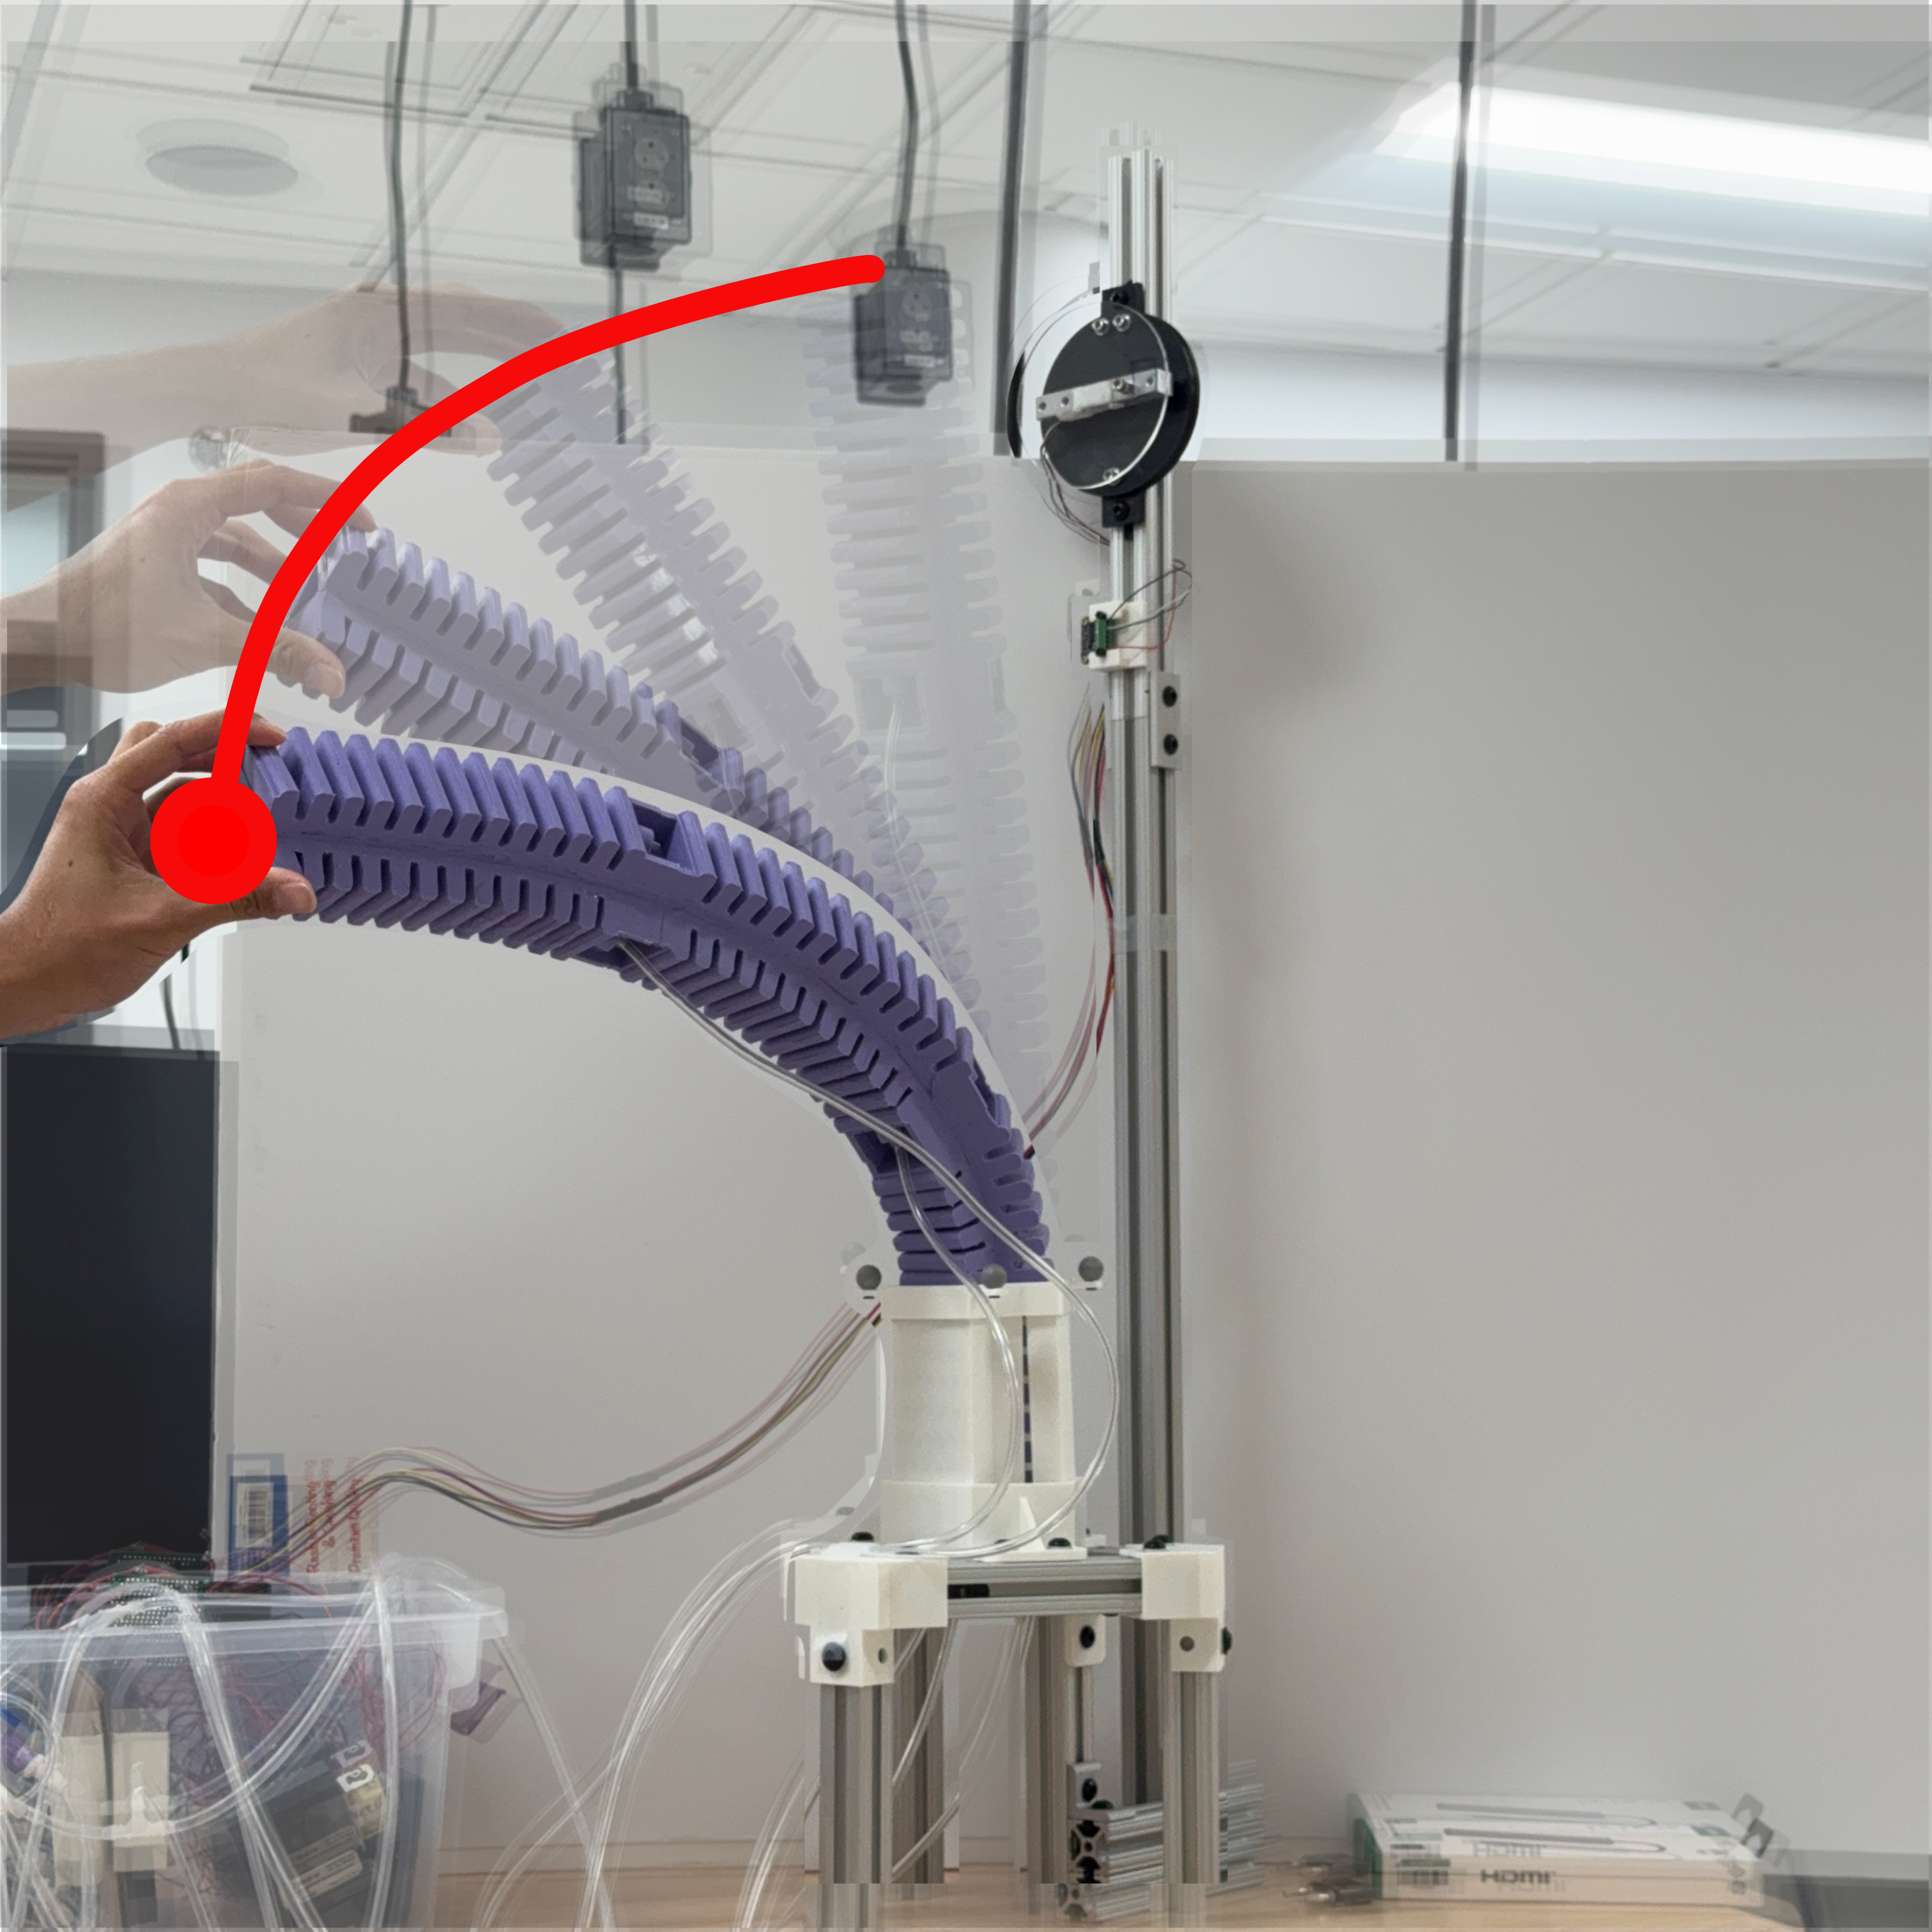
\includegraphics[width=0.6\textwidth]{graphics/trajDiag.PNG}
    \caption{The soft robot stabilizing around a trajectory}
    \label{taskspace}
\end{figure}

The test bench platform to be experimented on consists of: our pneumatically actuated soft robot, an Arduino-based system that handles the pressure actuation, an integrated codebase that manages communication between the Python-based dynamics computation and the Arduino-based actuation system, and finally a three-dimensional motion capture system. Using this platform, we will be able to closely assess the controller's performance. 

Our assessment methodology will revolve around the main functionalities being pursued. That is, we will assess the controller's performance based on its accuracy and stability. Practically speaking, this will involve building a dataset to serve as the reference configurations/trajectories, simulating what the system output looks like when using that dataset as the reference for our control input, running the control inputs from the dataset on our hardware, and finally comparing the results. Building the reference dataset will be done using the motion capture system: the soft robot's end effector can be pointed to various configurations or traced around different trajectories (like \autoref{taskspace}), "manually". Similarly, the configurations and trajectories that end up being physically achieved by the robot via the control inputs will be recorded using the motion capture system. This way, we can compare the reference and actual configurations and trajectories on the same measurement/recording platform.

\begin{comment}
    As the controller takes shape, simulations will then be run by implementing the controller onto the dynamic model. At this point, we are interested in seeing how closely does the output of the system come to the desired/reference configuration $\mathbf{r}$ when using the input signal $\mathbf{u}=f(\mathbf{x,r,e,t,...})$ produced by the controller. The big focus of this proposed thesis remains hardware implementation, but this phase includes a simulation step essentially as a validation method. The simulations should point out any glaring limitations or discrepancies in the controller formulated. 
\end{comment}